\documentclass{jacow}

\usepackage{graphicx}       % Extended support for \includegraphics
\usepackage{tikz}           % Powerful drawing package, part of pgf

\usepackage{mathptmx}       % Mathematical PostScript fonts
\usepackage{amsmath}        % General mathematical symbols
\usepackage{textcomp}       % Text companion fonts

\usepackage{url}            % \url command for decent line breaks in urls
\usepackage{enumitem}       % For more control over list parameters.


% PGF and TikZ definitions for this paper

% TikZ library imports
\usetikzlibrary{positioning}        % Anchor placement support
\usetikzlibrary{calc}               % Coordinate calculations
\usetikzlibrary{shapes.geometric}   % cylinder
\usetikzlibrary{shapes.arrows}      % arrow shapes
\usetikzlibrary{shapes.multipart}
\usetikzlibrary{fit}                % Fitting outline to shape
\usetikzlibrary{arrows}


% Define our colours
\colorlet{normal colour}{green!60!blue!20}  % Normal coloured filled areas
\colorlet{accent colour}{orange!20}         % Accented filled areas
\colorlet{background colour}{black!15}      % Background groups
\colorlet{data colour}{black!50}            % Data flow
\colorlet{control colour}{blue!50}          % Other lines etc


% Common TikZ definitions
\tikzset{
    % This seems a reasonably comfortable arrow shape
    >=stealth,
%
    % Define a set of styles
    % First some fills
    background fill/.style={fill=background colour},
    highlight fill/.style={fill=normal colour},
    accent fill/.style={fill=accent colour},
    % Next some lines
    bus/.style={color=data colour, text=black, line width=0.6mm, ->},
    control/.style={color=control colour, text=black, very thick, ->},
%
    % Used for creating an exact fit to an existing list of objects
    tight fit/.style={fit=#1, inner sep=0, line width=0},
    % We almost always want centre aligned node text
    every node/.style={align=center},
}


% New tikz key definitions to control behaviour of \multipath.
\tikzset{
    % Default colour for multipath background
    multipath background/.initial=white,
    multipath margin/.initial=0.3mm,
}

% Draws multiple paths with an outline on each path.  Call with path options as
% first optional argument and with a list of paths as the second argument.
\newcommand{\multipath}[2][]{
    \begin{scope}[#1]
        % Pick up multipath margin and background definitions
        \newcommand{\margin}{\pgfkeysvalueof{/tikz/multipath margin}}
        \newcommand{\background}{\pgfkeysvalueof{/tikz/multipath background}}

        % Draw a white background a bit larger than the programmed line
        % thickness.  We turn off any arrows and shorten the line a trifle to
        % avoid any erosion of the endpoints.
        \begin{scope}[
            line width=\pgflinewidth+\margin, color=\background,
            shorten >=\margin, shorten <=\margin, -]
        #2
        \end{scope}

        % Now draw the target path with its original options.
        #2
    \end{scope}
}


% It's convenient to have a background layer
\pgfdeclarelayer{background}
\pgfsetlayers{background,main}



% vim: set filetype=tex:
     % PGF & TikZ configuration


\hyphenpenalty 4000         % Tone down hyphenation.

% Tricky hack to make the last line of each caption aligned.  This is ... umm ..
% perhaps not altogether necessary, but I like the result.
\newcommand{\squarecaption}[2][1]{\caption[#1]{#2\unskip\parfillskip 0pt}}


\begin{document}
\title{ARCHITECTURE OF TRANSVERSE MULTI-BUNCH FEEDBACK PROCESSOR AT DIAMOND}
\author{M.G.~Abbott, G.~Rehm, I.S.~Uzun, Diamond Light Source, Oxfordshire, UK}
\maketitle


\begin{abstract}

We describe the detailed internal architecture of the Transverse Multi-Bunch
Feedback processor used at Diamond for control of multi-bunch instabilities and
measurement of betatron tunes.  Bunch by bunch selectable control over
feedback filters, gain and excitation allows fine control over feedback,
allowing for example the single bunch in a hybrid or camshaft fill pattern to
be controlled independently from the bunch train.  It is also possible to
excite all bunches at a single frequency while simultaneously sweeping the
excitation for tune measurement of a few selected bunches.  The single
frequency excitation has been used for continuous measurement of the
beta-function.  A simple programmable event sequencer provides support for up
to 7 steps of programmable sweeps and changes to feedback and excitation,
allowing a variety of complex and precisely timed beam characterisation
experiments including grow-damp measurements in unstable conditions and
programmed bunch cleaning.  Finally input and output compensation filters
allow for correction of front end and amplifier phasing at higher frequencies.

\end{abstract}



\section{Introduction}

At Diamond Light Source (DLS) we have been using a Transverse Multi-Bunch
Feedback (TMBF) system based on the Libera hardware platform~\cite{libera} for
nearly a decade~\cite{dipac2007, epac2008, biw2010, icalepcs2011} to control
multibunch instabilities.  With a new bunch position every 2\,ns it is
appropriate for the feedback processing to be implemented in an FPGA.  The
original firmware was based on work done at the ESRF~\cite{epac2006}, but
subsequently the firmware and control system have been rewritten to provide
further extensions to the system functionality~\cite{ibic2013, ibic2014}.  This
work has extended the lifetime of the original platform and increased its
capability, and the DLS TMBF system has now been adopted at ALBA~\cite{ibic2015}
and is being evaluated at the Australian Synchrotron.

In this paper we expand on and update the original IBIC 2013~\cite{ibic2013}
paper with many system refinements.



\section{Overview}

\begin{figure}[ht]
\begin{centering}
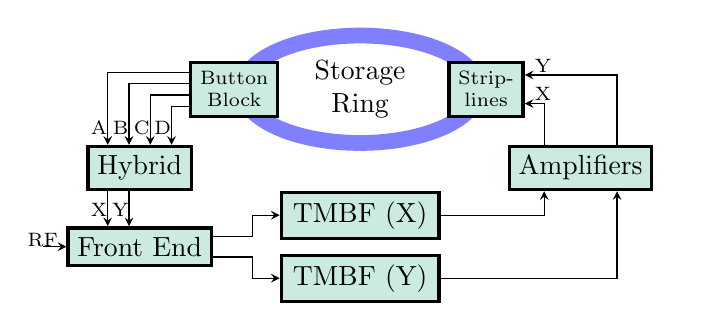
\begin{tikzpicture}[
    box/.style={draw, very thick, highlight fill},
    small box/.style={box, font=\scriptsize},
    small label/.style={font=\scriptsize, inner sep=0},
    ]

% This path defines the extent of the diagram to ensure it's centered nicely.
\path (-4,0) (4,0);

% Storage ring
\node (sr) [
    draw, control colour, text=black, ellipse,
    line width=2mm, minimum width=30mm] {Storage\\Ring};

\node [small box] (bpm) at (sr.west) {Button\\Block};

% Hybrid circuit converting BPM ABCD to XYSQ
\node [box] (hybrid) at (-2.8,-1) {Hybrid};
\foreach \p/\n in {0.2/A, 0.4/B, 0.6/C, 0.8/D} {
    \draw [->]
        ($(bpm.north west)!\p!(bpm.south west)$) -|
        ($(hybrid.north west)!\p!(hybrid.north east)$)
        node [small label, above left] at +(0,0.8ex) {\n}; }

% Front end
\node [box] (front end) at (-2.8,-2) {Front End};
\newcommand{\hybridfe}[2]{
    \draw [->]
        let \p1=($(hybrid.south west)!#1!(hybrid.south east)$) in
        (\p1) -- (front end.north -| \p1)
        node [small label, above left] at +(0,0.8ex) {#2};}
\hybridfe{0.2}{X}
\hybridfe{0.4}{Y}
\draw [<-] (front end.west) -- ++(-3mm,0)
    node [small label, above] {RF};

\node [box, minimum width=20mm] (tmbf X) at (0,-1.6) {TMBF (X)};
\node [box, minimum width=20mm] (tmbf Y) at (0,-2.4) {TMBF (Y)};
\newcommand{\tmbfamp}[2]{
    \draw [->]
    ($(front end.north east)!#1!(front end.south east)$) --
    +(0.5,0) |- (tmbf #2);
}
\tmbfamp{0.25}{X}
\tmbfamp{0.75}{Y}

% Amplifiers
\node [box] (amplifier) at (2.8,-1) {Amplifiers};
\draw [->] (tmbf X) -| ($(amplifier.south west)!0.25!(amplifier.south east)$);
\draw [->] (tmbf Y) -| ($(amplifier.south west)!0.75!(amplifier.south east)$);

% Striplines driving beam
\node [small box] (stripline) at (sr.east) {Strip-\\lines};
\foreach \p/\n in {0.25/X, 0.75/Y} {
    \draw [->]
        ($(amplifier.north west)!\p!(amplifier.north east)$) |-
        ($(stripline.south east)!\p!(stripline.north east)$)
        node [small label, above right] at +(0.8ex, 0.2ex) {\n};}

\end{tikzpicture}

% vim: filetype=tex:

\end{centering}
\squarecaption{
TMBF system in context.  The Transverse Multi-Bunch Feedback system measures the
position of each bunch, detects the betatron oscillations of each bunch, and
generates a drive signal to suppress the oscillations.
}
\label{context}
\end{figure}


\begin{figure}[ht]
\begin{centering}
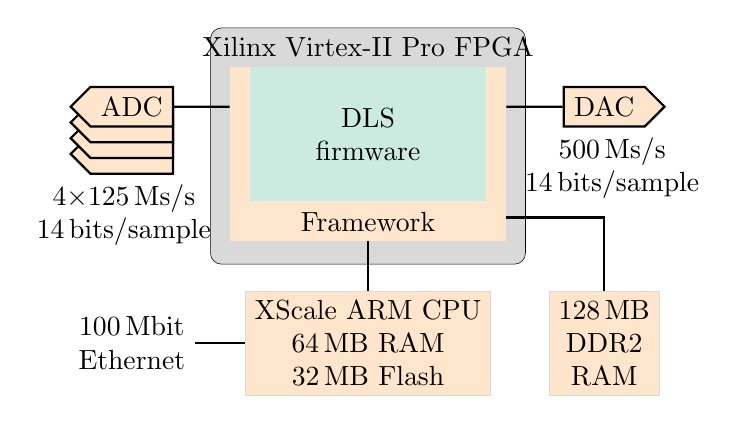
\begin{tikzpicture}[
    adc-dac/.style={
        draw, single arrow, thick, accent fill,
        single arrow head extend=0pt, shape border rotate=#1},
    outline/.style={draw=background colour, very thin},
    ]

\draw (-3,-0.6)
    node [adc-dac=180,
        label={[xshift=-1mm]below:4$\times$125\,Ms/s\\14\,bits/sample}]
        {\phantom{ADC}} ++(0,0.2)
    node [adc-dac=180] {\phantom{ADC}} ++(0,0.2)
    node [adc-dac=180] {\phantom{ADC}} ++(0,0.2)
    node (adc) [adc-dac=180] {ADC};

    \draw (3,0) node (dac) [
        adc-dac=0, label={[xshift=1mm]below:500\,Ms/s\\14\,bits/sample}]
        {DAC};

\path (0,-0.5)
    node (fpga) [
        outline, black,
        rectangle, fill=background colour, rounded corners,
        minimum height=30mm, minimum width=40mm] {}
    node [anchor=north] at (fpga.north) {Xilinx Virtex-II Pro FPGA}
    node (neutrino) [
        rectangle, accent fill,
        minimum height=22mm, minimum width=35mm] at +(0,-1mm) {}
    node [anchor=south] at (neutrino.south) {Framework}
    node [
        rectangle, highlight fill,
        minimum height=17mm, minimum width=30mm] at +(0,1.5mm) {DLS\\firmware};

\path
    (0,-3) node (arm) [outline, rectangle, accent fill]
        {XScale ARM CPU\\64\,MB RAM\\32\,MB Flash}
    (3,-3) node (ram) [outline, rectangle, accent fill]
        {128\,MB\\DDR2\\RAM}
    (-3,-3) node (ethernet) {100\,Mbit\\Ethernet};

\draw [thick] (adc) -- (neutrino.west |- adc);
\draw [thick] (dac) -- (neutrino.east |- dac);
\draw [thick] (neutrino) -- (arm);
\draw [thick] (neutrino.south east) +(0,3mm) -| (ram);
\draw [thick] (ethernet) -- (arm);

\end{tikzpicture}

% vim: filetype=tex:

\end{centering}
\squarecaption{
Libera System Platform.  The DLS TMBF system is implemented on the
Instrumentation Technologies Libera platform with the control system running
EPICS on an ARM based embedded Single Board Controller (SBC).
}
\label{system}
\end{figure}


Figure \ref{context} shows the TMBF processors in context.  A 4-button electrode
assembly together with an RF hybrid circuit picks up the horizontal and vertical
position of each bunch.  An RF front end converts this raw 3rd harmonic signal
into a 250\,MHz bandwidth bunch position signal suitable for processing by TMBF.
This signal is digitised at 500\,MHz (using four 125\,MHz ADCs phased at 2\,ns
intervals), processed by the FPGA, and then reconverted to drive the striplines.

The position of each bunch oscillates at the machine betatron tune, and these
oscillations can normally be suppressed by feeding them back with a phase shift
of 180\textdegree.  The TMBF measures the horizontal or vertical position of
each bunch, runs a 10-tap FIR filter on each bunch position to compute the
appropriate phase adjustment, and outputs a negative feedback signal.

The TMBF processing system consists of analogue to/from digital converters
connected to an FPGA for the high speed processing, together with memory for
data capture and an embedded Single Board Computer as shown in
Fig.~\ref{system}.

As well as the core feedback function, a number of diagnostic functions are
provided, both to enable easy monitoring of the system status, and to support
complex experiments on the beam.  System status monitoring includes detailed
overflow detection and quick measurement of beam movement.  Complex experiments
are supported by internal oscillators, detectors, and a programmable sequencer,
described in more detail below.


\begin{figure*}[t]
\begin{centering}
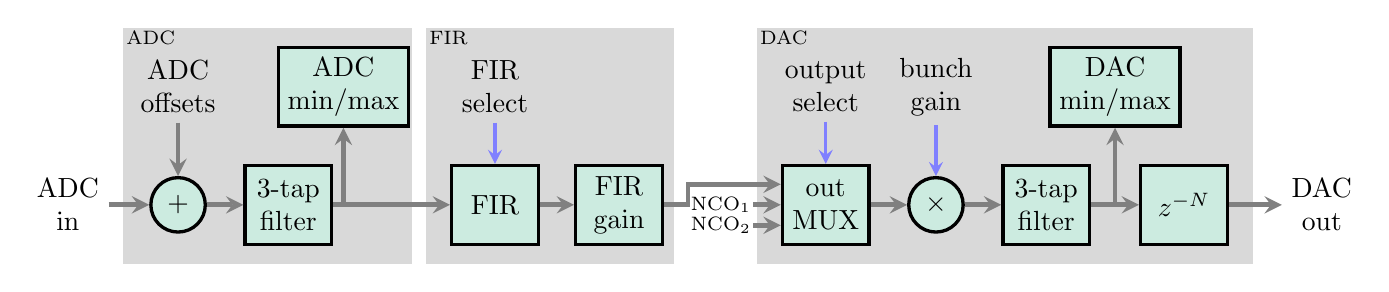
\begin{tikzpicture}[
    box/.style={draw, rectangle, very thick, highlight fill,
        minimum width=11mm, minimum height=10mm},
    mul/.style={draw, circle, very thick, highlight fill},
    area label/.style={anchor=north west, font=\scriptsize, inner sep=1pt},
    nco label/.style={anchor=east, font=\scriptsize, inner sep=0},
    x=1.75cm, y=1.5cm,
]

\path [background fill] (0.4,1.5) coordinate (adc top) rectangle ++(2.1,-2);
\path [background fill] (2.6,1.5) coordinate (fir top) rectangle ++(1.8,-2);
\path [background fill] (5.0,1.5) coordinate (dac top) rectangle ++(3.6,-2);
\path
    (adc top) node [area label] {ADC}
    (fir top) node [area label] {FIR}
    (dac top) node [area label] {DAC};

\path
    (0,0) node (adc in) {ADC\\in}
    ++(0.8,0) node (add offsets) [mul] {$+$}
    +(0,1) node (offsets) {ADC\\offsets}
    ++(0.8,0) node (adc filter) [box] {3-tap\\filter}
    ++(0.4,0) +(0,1) node (adc minmax) [box] {ADC\\min/max}
    ++(1.1,0) node (fir) [box] {FIR}
    +(0,1) node (fir select) {FIR\\select}
    ++(0.9,0) node (fir gain) [box] {FIR\\gain}
    ++(1.5,0) node (mux) [box] {out\\MUX}
    +(0,1) node (mux select) {output\\select}
    ++(0.8,0) node (add gain) [mul] {$\times$}
    +(0,1) node (gain) {bunch\\gain}
    ++(0.8,0) node (dac filter) [box] {3-tap\\filter}
    ++(0.5,0) +(0,1) node (dac minmax) [box] {DAC\\min/max}
    ++(0.5,0) node (delay) [box] {$z^{-N}$}
    ++(1,0) node (dac out) {DAC\\out};

\draw [bus] (adc in) -- (add offsets);
\draw [bus] (offsets) -- (add offsets);
\draw [bus] (add offsets) -- (adc filter);
\draw [bus] (adc filter) -| (adc minmax);
\draw [control] (fir select) -- (fir);
\draw [bus] (adc filter) -- (fir);
\draw [bus] (fir) -- (fir gain);
\draw [control] (mux select) -- (mux);
\draw [bus] (mux) -- (add gain);
\draw [control] (gain) -- (add gain);
\draw [bus] (add gain) -- (dac filter);
\draw [bus] (dac filter) -| (dac minmax);
\draw [bus] (dac filter) -- (delay);
\draw [bus] (delay) -- (dac out);

% Inputs to output mux need more care
\path (mux.north west) coordinate (mnw) (mux.south west) coordinate (msw);
\draw [bus] (fir gain) -- ++(0.5,0) |- ($(mnw)!0.25!(msw)$);
\draw [bus, <-] ($(mnw)!0.5!(msw)$) -- ++(-0.2,0)
    node [nco label] {NCO\textsubscript1};
\draw [bus, <-] ($(mnw)!0.75!(msw)$) -- ++(-0.2,0)
    node [nco label] {NCO\textsubscript2};

\end{tikzpicture}

% vim: filetype=tex:

\end{centering}
\squarecaption{
This is the core data processing chain in the TMBF processor.  Data processing
starts by adding a DC offset to each of the four ADC channels to compensate for
static ADC errors, followed by a 3-tap filter to compensate for high frequency
phase errors in the front end.  The minimum and maximum value per bunch of both
the ADC and DAC streams is captured for display.  A 10-tap filter with
programmable gain (in 6\,dB steps) is applied in turn to each bunch in the ring.
The output multiplexer adds any combination of its three inputs, which is then
scaled by a bunch specific gain.  Finally an output pre-emphasis filter corrects
for amplifier errors and is followed by a delay line to correctly close the
loop.
}
\label{data_chain}
\end{figure*}


\section{Feedback Data Processing}

The main function of TMBF is to stabilise transverse oscillations of the beam.
This is done by running a separate 10-tap FIR on the position of each of the
stored bunches.  The core data processing chain shown in Fig.~\ref{data_chain}
combines this feedback with up to two optional Numerically Controlled Oscillator
(NCO) outputs.

Note that numerical overflow can occur at any stage in this processing chain.
When this is detected, a saturated output is generated and the resulting
overflow event is reported to the user through the EPICS interface.


\subsection{ADC data in}

The Libera platform uses four separate 125\,MHz ADCs to sample the 500\,MHz
bunch position signal, and so the ADC input arrives as four parallel streams of
125\,MHz data.  The first processing step is to compensate for small DC offsets
between the ADCs.  These offsets are easily measured and compensated.

The next step is to compensate for gain differences and high frequency phase and
gain errors in the front end.  This is done by running a channel dependent 3-tap
filter on the input data stream.

Finally a ``min/max'' subunit measures the minimum and maximum compensated value
for each bunch; this is read out at 100\,ms intervals and used to provide an
accessible overview of bunch motion.


\subsection{FIR feedback processing}

Next a 10-tap FIR is run on the stream from each bunch.  In practice, this means
that 936 separate FIRs are run, with a delay of 936 bunches between each tap.
The FIR unit can be programmed with four different filters, each of which can be
separately selected for each bunch.  The filter taps and final output gain are
statically configured through the EPICS interface.

The ability to control bunches independently has two main uses: firstly, it can
be used to apply a different filter to the isolated bunch in a hybrid fill;
secondly, it can be useful as part of detailed machine physics experiments.


\subsection{DAC data out}

Finally the filtered signal is prepared for output.  At this point three
candidate output signals are selected and summed together: the FIR filtered
signal and two internally generate NCO signals.  Each of these three signals can
be output or set to zero, and this control is per bunch.

Next the summed output is scaled by a bunch specific scaling factor.  As this is
signed it can be used to reverse the orientation of feedback on a single bunch.

Finally an output pre-emphasis filter is run to compensate for amplifier effects
and the output is delayed so that the complete loop delay is a full machine
revolution.

In the same way for ADC data, a ``min/max'' component measures the movement of
each output bunch over a measurement interval of 100\,ms, providing a quick view
of bunch output motion.


\begin{figure}[t]
\begin{centering}
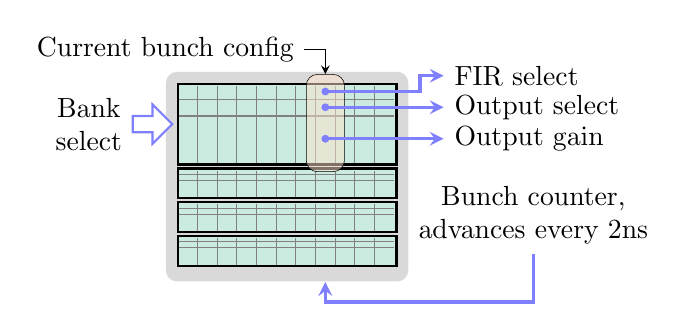
\begin{tikzpicture}[
    basic node/.style={draw, highlight fill, thick},
    cursor/.style={
        accent fill, rounded corners, draw, very thin, fill opacity=0.5},
    grid lines/.style={draw, thin, gray},
]

\newcommand{\horizspace}{2.5mm}
\newcommand{\horizcount}{10}
\newcommand{\cursorcount}{7}

% Draw four memory banks, the last one the largest
\path (0,0) coordinate (bank);
\foreach \hhh in {3.5mm, 3.5mm, 3.5mm, 10mm}
{
    \node [
        anchor=south, yshift=0.5mm,
        basic node, draw=none, rectangle, inner sep=0,
        minimum width=\horizspace*(\horizcount+1), minimum height=\hhh,
    ] (bank) at (bank.north) {};
    \foreach \xx in {1,...,\horizcount}{
        \draw [grid lines]
        ($(bank.south west)+\xx*(\horizspace,0)$) -- ++(0,\hhh);
    }
    \foreach \yy in {0.2, 0.4} {
        \draw [grid lines]
        let \n1={\horizspace*(\horizcount+1)} in
        ($(bank.north west)!\yy!(bank.south west)$) -- ++(\n1,0);
    }
    \draw [thick] (bank.north west) rectangle (bank.south east);
}

% Define and draw the cursor, label the components
\path let
    \p1=($(bank.north west)+\cursorcount*(\horizspace,0)$),
    \p2=($(\p1)+(\horizspace,-10mm)$) in
    node [rectangle, tight fit={(\p1) (\p2)}] (cursor) {};
\node [cursor, fit={(cursor)}] (cursor highlight) {};

\foreach \vpos/\voff/\name in {
    0.1/0.2/FIR select, 0.3/0/Output select, 0.7/-0.0/Output gain}
{
    \draw [control]
        ($(cursor.north)!\vpos!(cursor.south)$)
        node [circle, fill=control colour, inner sep=0, minimum size=1mm] {}
        coordinate (p) -- (p -| bank.east)
        -- ++(3mm,0) -- ++(0,\voff) -- ++(3mm,0)
        node [anchor=west] {\name};
}

\begin{pgfonlayer}{background}
    \node [rectangle, background fill, rounded corners,
        fit={(0,0) (bank)}, inner sep=1.5mm] (memory) {};
\end{pgfonlayer}

\draw
    (bank.west) node [
        xshift=-0.5mm,
        draw, thick, control colour, fill=white,
        single arrow, anchor=east, inner sep=0,
        minimum height=5mm, minimum width=5mm,
        single arrow head extend=0.2mm] (select) {}
    node [anchor=east] at (select.west) {Bank\\select};

\path (memory.north west) node [anchor=south] (current) {Current bunch config};
\draw [->] (current) -| (cursor highlight);

\path (memory.east) node [
anchor=north west] (counter) {Bunch counter,\\advances every 2ns};
\draw [control] (counter) -- ++(0,-1.1cm) -| (memory.south -| cursor);

\end{tikzpicture}

% vim: filetype=tex:

\end{centering}
\squarecaption{
Bunch by bunch FIR and output control.  The sequencer selects one of four banks
to be active, defining basic machine behaviour.  Each bank contains bunch
configuration information for each of the stored bunches, used to control the
feedback filter and the output configuration.
}
\label{bunch}
\end{figure}

\subsection{Bunch by Bunch Control}

As noted above, the FIR filter, the output sum, and the final output gain are
selected per bunch.  The ``Bunch Select'' unit, see Fig.~\ref{bunch}, stores
four arrays (or ``banks'') of bunch specific configurations --- one
configuration is selected by the sequencer unit (described below), and the
current bunch configuration advances on each bunch.  This configuration can be
written through the EPICS interface.


\begin{figure*}[!ht]
\begin{centering}
\newcommand{\westcoord}[3]{
    \coordinate (#1 #2) at ($(#1.south west)!#3!(#1.north west)$)}
\newcommand{\eastcoord}[3]{
    \coordinate (#1 #2) at ($(#1.south east)!#3!(#1.north east)$)}

\begin{tikzpicture}[
    box/.style={
        draw, rectangle, very thick, highlight fill,
        minimum width=1.8cm, minimum height=1.5cm},
    adc-dac/.style={
        draw, single arrow, very thick, accent fill,
        inner ysep=2mm,
        single arrow head extend=0pt, shape border rotate=#1},
    wide box/.style={minimum width=3cm},
    tall box/.style={minimum height=3cm},
    trigger/.style={semithick, >=open triangle 60, shorten >=-6pt, ->},
    x=2cm, y=2.3cm]

    % ADC input node
    \node [adc-dac=180] (ADC) at (-1,0) {ADC};
    \node [box] (adc) at (0,0) {ADC};
    \draw [bus] (ADC) -- (adc);
    \draw [bus, -] (ADC.west) -- +(-4mm,0);

    % FIR processing node
    \node [box] (fir) at (1.5,0) {FIR};

    % DAC output node
    \path node [box] (dac) at (5,0) {} (dac.east) node [anchor=east] {DAC};
    \westcoord{dac}{fir in}{0.75};
    \westcoord{dac}{nco1 in}{0.5};
    \westcoord{dac}{nco2 in}{0.25};
    \eastcoord{dac}{out}{0.2};
    \node [adc-dac=0] (DAC) at ($(dac)+(1,0)$) {DAC};
    \draw [bus] (dac) -- (DAC);
    \draw [bus, -] (DAC.east) -- +(4mm,0);
    \path [font=\scriptsize, anchor=west]
        (dac fir in) node {FIR}
        (dac nco1 in) node {NCO\textsubscript1}
        (dac nco2 in) node {NCO\textsubscript2};

    % Two NCO processing nodes
    \newcommand{\nco}[3]{
        \node [box, wide box] (#1) at #2 {#3};
        \westcoord{#1}{adc in}{0.25};
        \westcoord{#1}{fir in}{0.75};
        \eastcoord{#1}{iq out}{0.25};
        \eastcoord{#1}{nco out}{0.75};
        \path [font=\scriptsize, anchor=west]
            (#1 adc in) node {ADC}
            (#1 fir in) node {FIR};
        \path [font=\scriptsize, anchor=east]
            (#1 nco out) node {NCO}
            (#1 iq out) node {IQ};
    }
    \nco{nco1}{(2.5,-1)}{NCO\textsubscript{1} \&\\Tune PLL}
    \nco{nco2}{(2.5,-2)}{NCO\textsubscript{2} \&\\Sequencer}

    % Bunch selection centred above FIR and DAC with control signals
    \node [box, minimum height=1.2cm] (bunch) at (2.8,0.8) {Bunch\\Select};

    % Data capture output node
    \node [box, wide box, tall box] (capture) at (5.6,-1.5) {Data\\Capture};
    \westcoord{capture}{dac in}{0.8};
    \westcoord{capture}{fir in}{0.7};
    \westcoord{capture}{adc in}{0.6};
    \westcoord{capture}{iq1 in}{0.35};
    \westcoord{capture}{iq2 in}{0.25};
    \path [font=\scriptsize, anchor=west]
        (capture dac in) node {DAC}
        (capture fir in) node {FIR}
        (capture adc in) node {ADC}
        ($(capture iq1 in)!0.5!(capture iq2 in)$) node {IQ};

    % Triggering of sequencer and data capture
    \node [box] (trigger) at (0,-2) {Triggers};
    \draw [thick, font=\scriptsize, anchor=east]
        ($(trigger.south west)!0.75!(trigger.north west)$) -- ++(-4mm,0)
            node {TRG}
        ($(trigger.south west)!0.5!(trigger.north west)$) -- ++(-4mm,0)
            node {PM}
        ($(trigger.south west)!0.25!(trigger.north west)$) -- ++(-4mm,0)
            node {SCLK};
    \draw [trigger, -]
        let \p1 = (trigger |- capture), \p2 = ($(\p1)+(0.6,0)$) in
        (trigger) -- ($(trigger)+(0.6,0)$) -- (\p2) coordinate (trigger p);
    \draw [trigger] (trigger p) -- (capture);
    \draw [trigger, rounded corners] (trigger p) -| (nco1);
    \draw [trigger, rounded corners] (trigger p) -| (nco2);
    \draw [trigger] (trigger p) |- (bunch);

    % Bunch control signals: need to be drawn above triggers.
    \multipath[control] { \draw (nco2) -| (3.5,0) |- (bunch); }
    \node [anchor=south west, font=\small, text=black]
        at (bunch.east) {bank select};
    \multipath[control] {
        \draw (bunch) -- (bunch |- 0,0.45) -| (fir);
        \draw (bunch) -- (bunch |- 0,0.45) -| (dac);
    }
    \node [anchor=south east, font=\small] at (fir.north) {FIR\\select};
    \node [anchor=south west, font=\small] at (dac.north)
        {output select\\\& bunch gain};

    % SBC control
    \node [box] at (0,-1.25) {SBC\\Interface};

    % ADC outputs to FIR, detectors and capture
    \coordinate (adc fir) at ($(adc)!0.5!(fir)$);
    \multipath[bus] {
        \draw (adc) -- (fir);
        \draw (adc fir) |- (nco1 adc in);
        \draw (adc fir) |- (nco2 adc in);
        \draw (adc fir) -- ++(0,-0.5) -- (4.1,-0.5) |- (capture adc in);
    }

    % FIR to DAC and capture
    \multipath[bus] {
        \draw (fir) -| (dac fir in -| 3, 0) -- (dac fir in);
        \draw (dac fir in -| 4.3, 0) |- (capture fir in);
    }

    % Captured DAC out
    \multipath[bus] {
        \draw (dac out) -- (dac out -| 5.6,0) |- (4.5,-0.5) |- (capture dac in);
    }
    % Captured IQ
    \multipath[bus] {
        \draw (nco1 iq out) -- (nco1 iq out -| 3.7,0) |- (capture iq1 in);
        \draw (nco2 iq out) -- +(1,0) |- (capture iq2 in); }

    % DAC NCO inputs
    \multipath[bus] {
        \draw (nco1 nco out) -- (nco1 nco out -| 3.7,0) |- (dac nco1 in); }
    \multipath[bus] {
        \draw (nco2 nco out) -- (nco2 nco out -| 3.9,0) |- (dac nco2 in); }

    % High resolution FIR inputs to detectors
    \multipath[bus] {
        \draw (fir) |- (nco1 fir in);
        \draw (fir) |- (nco2 fir in);
    }

\end{tikzpicture}

% vim: filetype=tex:

\end{centering}
\squarecaption[fragile]{
Here we see all of the major blocks of the FPGA system design and their
data interconnections.  FPGA blocks are shown thus: \tikz \node [draw,
rectangle, thick, highlight fill] {}; and analogue/digital converters
thus: \tikz \node [draw, thick, fill=orange!20, single arrow, single arrow head
extend=0] {};.  The main data flow is from the ADC, through the FIR with a
separate FIR filter selected for each bunch, and out through the DAC with the
option of adding up to two internally generated sine waves.  The other paths are
for control and data capture.  The SBC interface controls and communicates with
all other components of the system: the EPICS interface is through this
component.
}
\label{overview}
\end{figure*}


\section{Extra Diagnostic Data Processing}

Figure~\ref{overview} shows the complete DLS TMBF firmware.  The ADC-FIR-DAC
chain has been described above.  The remaining major components are for extra
diagnostics and advanced machine experiments.

\subsection{Data Capture}

As already shown, min/max overview data is available for ADC input and DAC
output.  The Data Capture unit allows more detailed information: up to 4096
bunches of two out of three of DAC/FIR/ADC data streams can be captured, or up
to 64 million bunches (more than 65,000 turns) of any one input can be captured.
The shorter data capture is to FPGA block memory, the larger to external DDR2
RAM.

An alternative capture source is detector IQ data from either of the two NCO
units.  In particular, this is used for tune sweeps and more complex machine
experiments.


\begin{figure}[hbt]
\begin{centering}
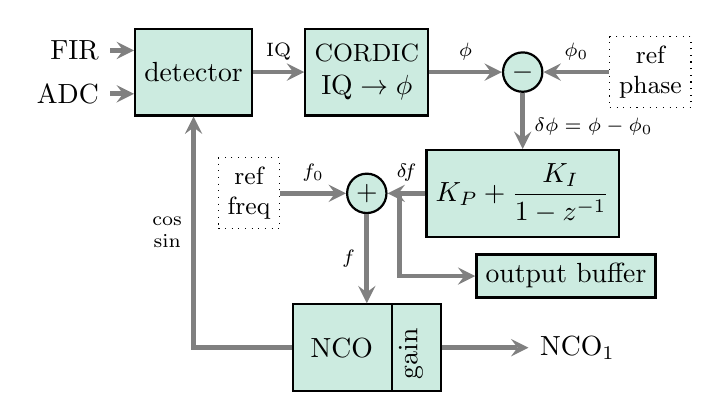
\begin{tikzpicture}[
    basic node/.style={draw, highlight fill, thick},
    box/.style={basic node, minimum height=11mm},
    add/.style={basic node, circle, minimum size=5mm, inner sep=0pt},
    mid above/.style={midway, above, font=\scriptsize},
    mid right/.style={midway, right, font=\scriptsize},
    ref value/.style={font=\small, draw, dotted},
    x=11mm, y=7mm,
]

\path
    node [box] (detector) {detector}
    ++(2,0) node [box] (cordic) {\small CORDIC\\$\text{IQ}\to\phi$}
    ++(1.8,0) node [add] (error) {$-$}
    ++(0,-2.2) node [box] (feedback) {$\displaystyle K_P+\frac{K_I}{1-z^{-1}}$}
    +(0.5,-1.5) node [basic node] (buffer) {output buffer}
    ++(-1.8,0) node [add] (f out) {$+$}
    ++(0,-2.8) node (nco) [
        box, rectangle split, rectangle split parts=2,
        rectangle split horizontal, inner sep=1.5ex] {NCO}
    (nco.two) node [rotate=90] {gain};


\draw [bus, <-] (detector.160) -- ++(-3mm,0) node[anchor=east] {FIR};
\draw [bus, <-] (detector.200) -- ++(-3mm,0) node[anchor=east] {ADC};

\draw [bus] (detector) -- (cordic) node [mid above] {IQ};
\draw [bus] (cordic) -- (error) node [mid above] {$\phi$};
\draw [bus, <-] (error) -- ++(1,0) node [mid above] {$\phi_0$} coordinate (p);
\node [anchor=west, ref value] at (p) {ref\\phase};
\draw [bus] (error) -- (feedback)
    node [mid right, pos=0.6] {$\delta\phi=\phi-\phi_0$};

\draw [bus] (feedback) -- (f out) node [mid above] {$\delta\!f$};
\draw [bus] (feedback.west) -- ++(-0.3,0) |- (buffer);
\draw [bus, <-] (f out) -- ++(-1,0) node [mid above] {$f_0$} coordinate(p);
\node [anchor=east, ref value] at (p) {ref\\freq};

\draw [bus] (f out) -- (nco) node [mid right, left] {$f$};
\draw [bus] (nco) -| (detector)
    node [near end, anchor=east, font=\scriptsize] {cos\\sin};

\draw [bus] (nco.east) -- ++(1,0) node [anchor=west] {NCO\textsubscript1};

\end{tikzpicture}

% vim: filetype=tex:

\end{centering}
\squarecaption{
The oscillator NCO\textsubscript1, can be set to a fixed frequency, or
can be used as part of a tune tracking phase locked loop.  The tune phase $\phi$
is measured at the operating frequency $f$ and used to compute a sequence of
frequency corrections $\delta\!f$ to maintain the phase error $\delta\phi$ at
zero.  The reference phase and frequency are configured via EPICS.
}
\label{nco1}
\end{figure}


\subsection{NCO\textsubscript1 and Tune PLL}

Figure~\ref{nco1} shows the first NCO unit together with the tune tracking
application (Tune PLL).  When tune tracking is inactive the NCO generates a
fixed frequency sine wave with programmable gain which can be used to drive
selected bunches.

When tune tracking is active the detector (see Fig.~\ref{nco2} for the detector
structure) measures the phase response of the beam at the currently driven
frequency and runs a simple PI feedback loop to adjust the frequency to keep the
phase response static.  The frequency shift can be read as a continuous stream
through the EPICS interface.

This is very useful for measuring rapid changes in the machine betatron
frequency, but will only work when the centre frequency and phase are already
known to sufficient precision.  Measuring this is the primary job of the next
unit.



\begin{figure}[hbt]
\begin{centering}
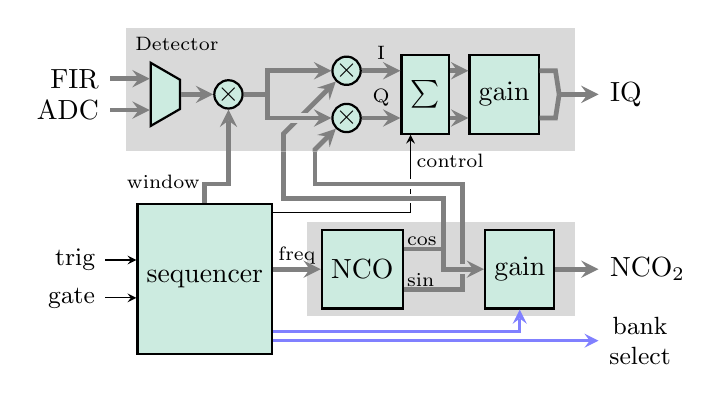
\begin{tikzpicture}[
    basic node/.style={draw, highlight fill, thick},
    mul/.style={basic node, circle, inner sep=0},
    tall box/.style={
        basic node, rectangle, minimum height=10mm, minimum width=6mm},
    y=6mm,
]


\path
    node [background fill, fit={(-0.5,1.4) (5.2,-1.2)}, inner sep=0]
        (detector) {}
    (detector.north west) node [anchor=north west, font=\scriptsize]
        {Detector};


\path
    (0,0) node [
        basic node, trapezium, shape border rotate=270,
        minimum width=8mm] (mux) {}
    ++(0.8,0) node [mul] (mul win) {$\times$}
    ++(1.5,0)
    +(0,0.5) node [mul] (mul I) {$\times$}
    +(0,-0.5) node [mul] (mul Q) {$\times$}
    ++(1,0) node [tall box] (sum) {$\sum$}
    ++(1,0) node [tall box] (det gain) {gain}
    ++(0.7,0) coordinate (iq node)
    ++(0.5,0) coordinate (iq);

\draw [bus, <-] (mux.north west) -- ++(-0.5,0) node[anchor=east] {FIR};
\draw [bus, <-] (mux.south west) -- ++(-0.5,0) node[anchor=east] {ADC};

\draw [bus] (mux) -- (mul win);
\draw [bus, <-]
    (mul I) -- ++(-8mm,-8mm) coordinate (p) -- (p |- detector.south)
    coordinate (det cos);
\draw [bus, <-]
    (mul Q) -- ++(-4mm,-4mm) coordinate (p) -- (p |- detector.south)
    coordinate (det sin);
\multipath [bus, multipath background=background colour] {
    \draw (mul win) -- ++(0.5, 0) |- (mul I);
    \draw (mul win) -- ++(0.5, 0) |- (mul Q);
}
\draw [bus] (mul I) -- (mul I -| sum.west)
    node [midway, anchor=south, font=\scriptsize] {I};
\draw [bus] (mul Q) -- (mul Q -| sum.west)
    node [midway, anchor=south, font=\scriptsize] {Q};
\draw [bus] (mul I -| sum.east) -- (mul I -| det gain.west);
\draw [bus] (mul Q -| sum.east) -- (mul Q -| det gain.west);
\draw [bus,-] (mul I -| det gain.east) -- ++(0.2,0) -- (iq node);
\draw [bus,-] (mul Q -| det gain.east) -- ++(0.2,0) -- (iq node);
\draw [bus] (iq node) -- (iq) node[anchor=west]{IQ};


\path [background fill] (1.8,-2.7) coordinate (nco top) rectangle +(3.4,-2);

% Place sequencer
\path (0.5,-2.3)
    node [tall box, anchor=north, minimum height=19mm] (seq) {sequencer};
\path
    (nco top)
    ++(0.7, -1) node [tall box] (nco) {NCO}
    ++(2,0) node [tall box] (nco gain) {gain}
    ++(1,0) coordinate (nco out);
\path
    ($(nco.north east)!0.25!(nco.south east)$) coordinate (cos)
    ($(nco.north east)!0.75!(nco.south east)$) coordinate (sin);
\draw [<-, font=\small]
    ($(seq.west)-(0,0.4)$) -- ++(-4mm,0) node [anchor=east] {gate};
\draw [<-, font=\small]
    ($(seq.west)+(0,0.4)$) -- ++(-4mm,0) node [anchor=east] {trig};

\draw [bus]
    (seq.east |- nco) -- (nco)
    node[pos=0, anchor=south west, font=\scriptsize, inner sep=1pt] {freq};
\draw [bus]
    (seq.north) -- ++(0,0.4)
    node[midway, anchor=south east, font=\scriptsize, inner sep=1pt] {window}
    -| (mul win);
\draw [->] ($(seq.north east)-(0,0.2)$) -| (sum.250)
    node[anchor=west, font=\scriptsize, inner sep=2pt, pos=0.83] {control};


\draw [bus, -]
    (sin) -- ++(0.75,0) coordinate (p) -- (p |- nco top) coordinate (nco sin);
\multipath[bus, multipath background=background colour] {
    \draw [-]
        (cos) -- ++(0.5,0) coordinate (p) -- (p |- nco top)
        coordinate (nco cos);
    \draw (cos) -- ++(0.5,0) |- (nco gain);
}
\multipath [bus, -] { \draw (nco cos) -- ++(0,0.5) -| (det cos); }
\multipath [bus, -] { \draw (nco sin) -- ++(0,0.8) -| (det sin); }

% Label the NCO outputs
\path
    (cos) node [anchor=south west, inner sep=1pt, font=\scriptsize] {cos}
    (sin) node [anchor=south west, inner sep=1pt, font=\scriptsize] {sin};


\draw [bus] (nco gain) -- (nco out) node[anchor=west] {NCO\textsubscript2};

\draw [control] ($(seq.south east)+(0,0.3)$) coordinate (p) -- (p -| nco out)
    node[anchor=west, font=\small] {bank\\select};
\draw [control] ($(seq.south east)+(0,0.5)$) -| (nco gain);


\end{tikzpicture}

% vim: filetype=tex:

\end{centering}
\squarecaption{
The oscillator NCO\textsubscript2 is under control of the sequencer, and is only
enabled while the sequencer is running a program.  The sequencer controls the
NCO frequency and gain and performs programmed frequency sweeps.  Data from the
beam is mixed with the excitation waveform  in the detector to measure a
complete complex IQ response.  Operation of this system produces a waveform of
IQ measurements which can be used for measuring betatron tune and other machine
parameters.
}
\label{nco2}
\end{figure}

\subsection{NCO\textsubscript2 and the Sequencer}

Figure~\ref{nco2} shows the second NCO unit together with the sequencer unit and
a detailed view of the detector.  The detector measures the complex response of
the selected input to the driving frequency.  The duration of each measurement
is controlled by the sequencer.  The measured IQ value is scaled to a pair of
16-bit numbers for storage and transferred to the control system.

The TMBF sequencer controls the NCO\textsubscript2 frequency, the
NCO\textsubscript2 output level, and which bunch bank is currently active.  A
machine experiment is performed by programming up to seven different control
configurations and then triggering the start of the sequencer.  The sequencer
will then work its way through the programmed states, changing the output
configuration as appropriate and capturing the appropriately programmed number
of IQ samples, before finishing.  Typically the sequencer and the data capture
unit are triggered together.

For example, a standard tune sweep is performed using a single sequencer state
which configures NCO\textsubscript2 for output and steps through a preset range
of NCO frequencies.  Alternatively, a grow-damp experiment requires more states:
one to excite the beam for a selected period, one to allow the beam to grow
without feedback or excitation for a period, and one to restore feedback.

One final feature of the sequencer is the so-called ``super-sequencer'': this
repeatedly performs a sequencer programme for a series of base frequencies.
This is used to perform a grow-damp experiment on each transverse mode in turn,
and allows the transverse mode damping times to be measured for all modes in a
fraction of a second~\cite{ibic2014}.


\section{EPICS Control System}

The control system running on the embedded ARM processor was developed
concurrently with the FPGA firmware, and provides access to all settings and
readings through around 560 EPICS PVs.  A number of supporting scripts were
written in Python and Matlab to help configure some of the more complex
functions of TMBF.

A complete set of user interface screens built using EDM provides access to
every PV published by TMBF.  Around 255 PVs are used to configure settings, so
the supporting scripts are important for normal operation.

The EPICS control system and the TMBF FPGA system are tightly coupled.  Although
the ARM processor is low powered and lacks hardware floating point support it is
capable of some signal processing if care is taken.  In particular, tune
measurement is done by first performing a frequency response sweep with the
FPGA, and then analysing the resulting IQ response and fitting a multi-pole tune
response model.  It has been possible to develop quite a sophisticated tune
measurement process on this system.


\section{Conclusions}

The upgraded TMBF system described here has been in use at Diamond since late
2013 and is allowing us to perform very complex measurements to characterise the
beam behaviour.  This development has pushed the 10 year old FPGA technology to
its limits, the FPGA now has little or no room for further developments.

Our next step at Diamond is to implement longitudinal bunch-by-bunch feedback in
preparation for operation with normally conducting cavities.  This will be based
on a more modern FPGA on industry standard MicroTCA hardware.


\begin{thebibliography}{9}

\bibitem{libera}
Instrumentation Technologies, \emph{Libera Bunch-by-Bunch},
\url{http://www.i-tech.si}.

\bibitem{dipac2007}
A.F.D.~Morgan, G.~Rehm, I.~Uzun, \emph{First Tests of the Transverse Multibunch
Feedback at Diamond}, DIPAC~2007.

\bibitem{epac2008}
A.F.D.~Morgan, G.~Rehm, I.~Uzun, \emph{Performance and Features of the Diamond
TMBF System}, EPAC~2008.

\bibitem{biw2010}
G.~Rehm, M.G.~Abbott, A.F.D.~Morgan, J.~Rowland, I.~Uzun, \emph{Measurement of
Lattice Parameters Without Visible Disturbance to User Beam at Diamond Light
Source}, BIW~2010.

\bibitem{icalepcs2011}
I.~Uzun, M.G.~Abbott, M.T.~Heron, A.F.D.~Morgan, G.~Rehm, \emph{Operational
Status of the Transverse Multibunch Feedback System at Diamond}, ICALEPCS~2011.

\bibitem{epac2006}
E.~Plouviez, P.~Arnoux, F.~Epaud, J.~Jacob, J.M.~Koch, N.~Michel, G.A.~Naylor,
J.\mbox{-}L.~Revol, V.~Serriere, D.~Vial, \emph{Broadband Bunch by Bunch
Feedback for the ESRF using a Single High Resolution and Fast Sampling FPGA
DSP}, EPAC~2006.

\bibitem{ibic2013}
M.G.~Abbott, G.~Rehm, I.S.~Uzun, \emph{Capability Upgrade of the Diamond
Transverse Multibunch Feedback}, IBIC~2013.

\bibitem{ibic2014}
G.~Rehm, M.G.~Abbott, A.F.D~Morgan, \emph{New Features and Measurements using
the Upgraded Transverse Multibunch Feedback at Diamond}, IBIC~2014.

\bibitem{ibic2015}
A.~Olmos, U.~Iriso, J.~Moldes, F.~P\'erez, M.~Abbott, G.~Rehm, I.~Uzun,
\emph{Integration of the Diamond Transverse Multibunch Feedback System at ALBA},
IBIC~2015.

% This is sometimes needed to work around a bug in the bibliography
\vspace{0pt}

\end{thebibliography}


\end{document}
